\documentclass[12pt,a4paper]{article}
  \usepackage[toc,page]{appendix}
  \usepackage{longtable}
  \usepackage{listings} 
  \usepackage{verbatim}
  \usepackage{graphicx}
  \usepackage{tabularx}
  \usepackage{subfig}
  \usepackage{float}
  \usepackage{pdfpages}
  \usepackage{csvsimple}
  \usepackage[a4paper,bindingoffset=0.2in,left=0.6in,right=0.6in,top=1in,bottom=1in,footskip=.25in]{geometry}
  \begin{document}
    \begin{titlepage}
      \centering
      {\scshape\LARGE Goldsmiths, University of London \par}
      \vspace{1cm}
      {\scshape\Large Software project final report\par}
      \vspace{1.5cm}
      {\huge\bfseries iLost\par}
      \vspace{2cm}
      {\Large\itshape 
        Ahmed, Muhammad\\
        Chowdhury, Thairan\\
        Davies Minta, Dylan\\     
        Fakrul, Mahmudul\\    
        Farkhani, Hussein\\ 
        Jheng-Hao, Lin\\
        Pecorella, Mariano\\ \par}
      \vfill
      supervised by\par
      \textsc{Tim Blackwell} 
      \vfill
      % Bottom of the page
      {\large \today \par}
    \end{titlepage}

    \tableofcontents
    \newpage

    \section{Introduction}
    \section{Development Record}
      \subsection{Technology Selection} 
        % 400 - 500 words
        During in the implementation stage, we setup a organisation {\bf GSoft} on Github and we were divided into three teams, {\bf iOS app}, {\bf Android app} and {\bf Backend/Tracker team}, which shows on the figure \ref{fig:Development Teams}. Each team was grouped by 2 to 3 people who were more interested in that topic or technology. Some of us were interested in more than two areas then he would join two of the teams. 

        \begin{figure}[H]
          \centering
          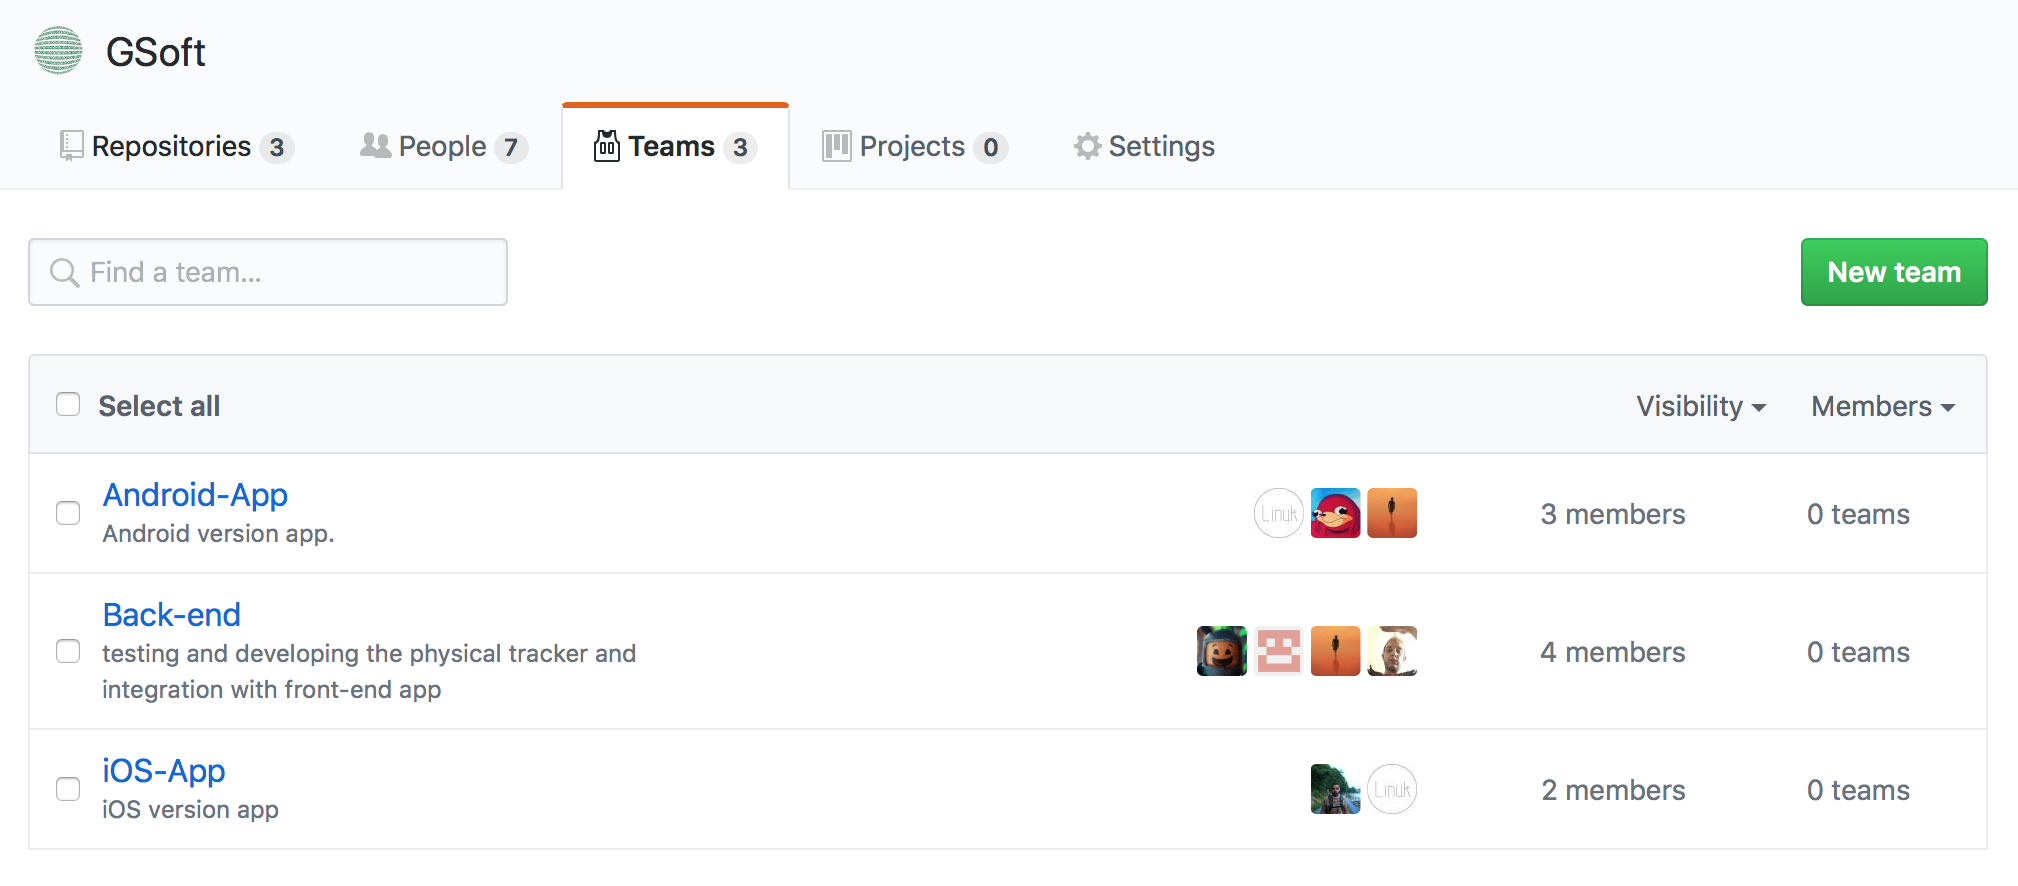
\includegraphics[width=1\textwidth]{../assets/development-records-teams.png}
          \caption{Development Teams}
          \label{fig:Development Teams}
        \end{figure}

        Each team was responsible for how and what technology to use as long as the production could be made on time. We believed this methodology had these advantages in terms of the limited development time:

        \begin{itemize}
          \item {React Agilely}:Compare to have a poll with all members of our group, it was agiler to come to the decision within 2 or 3 people within one team. Since each team could react to the situation and resolve the issues in a more efficient way.
          \item {Specialities differs}: Our group was divided by our interests and specialities, we trusted each team could make the best decision for the whole team with their research and experience. For example, the iOS app team would not interfere how tracker team implemented the physical components at all, and how Android app was implemented would not be the backend/tracker team's concern. All teams were trusted that they would make the best decisions.
        \end{itemize}
        
        Even though the team was separated, but it was important to keep everyone on the same page, so we used several channels on Slack to keep everyone updated. Such as the {\bf iOS channel} was be the place containing all updates related to iOS application development, which shows in figure \ref{fig:Slack iOS Channel}. 
        
        \begin{figure}[H]
          \centering
          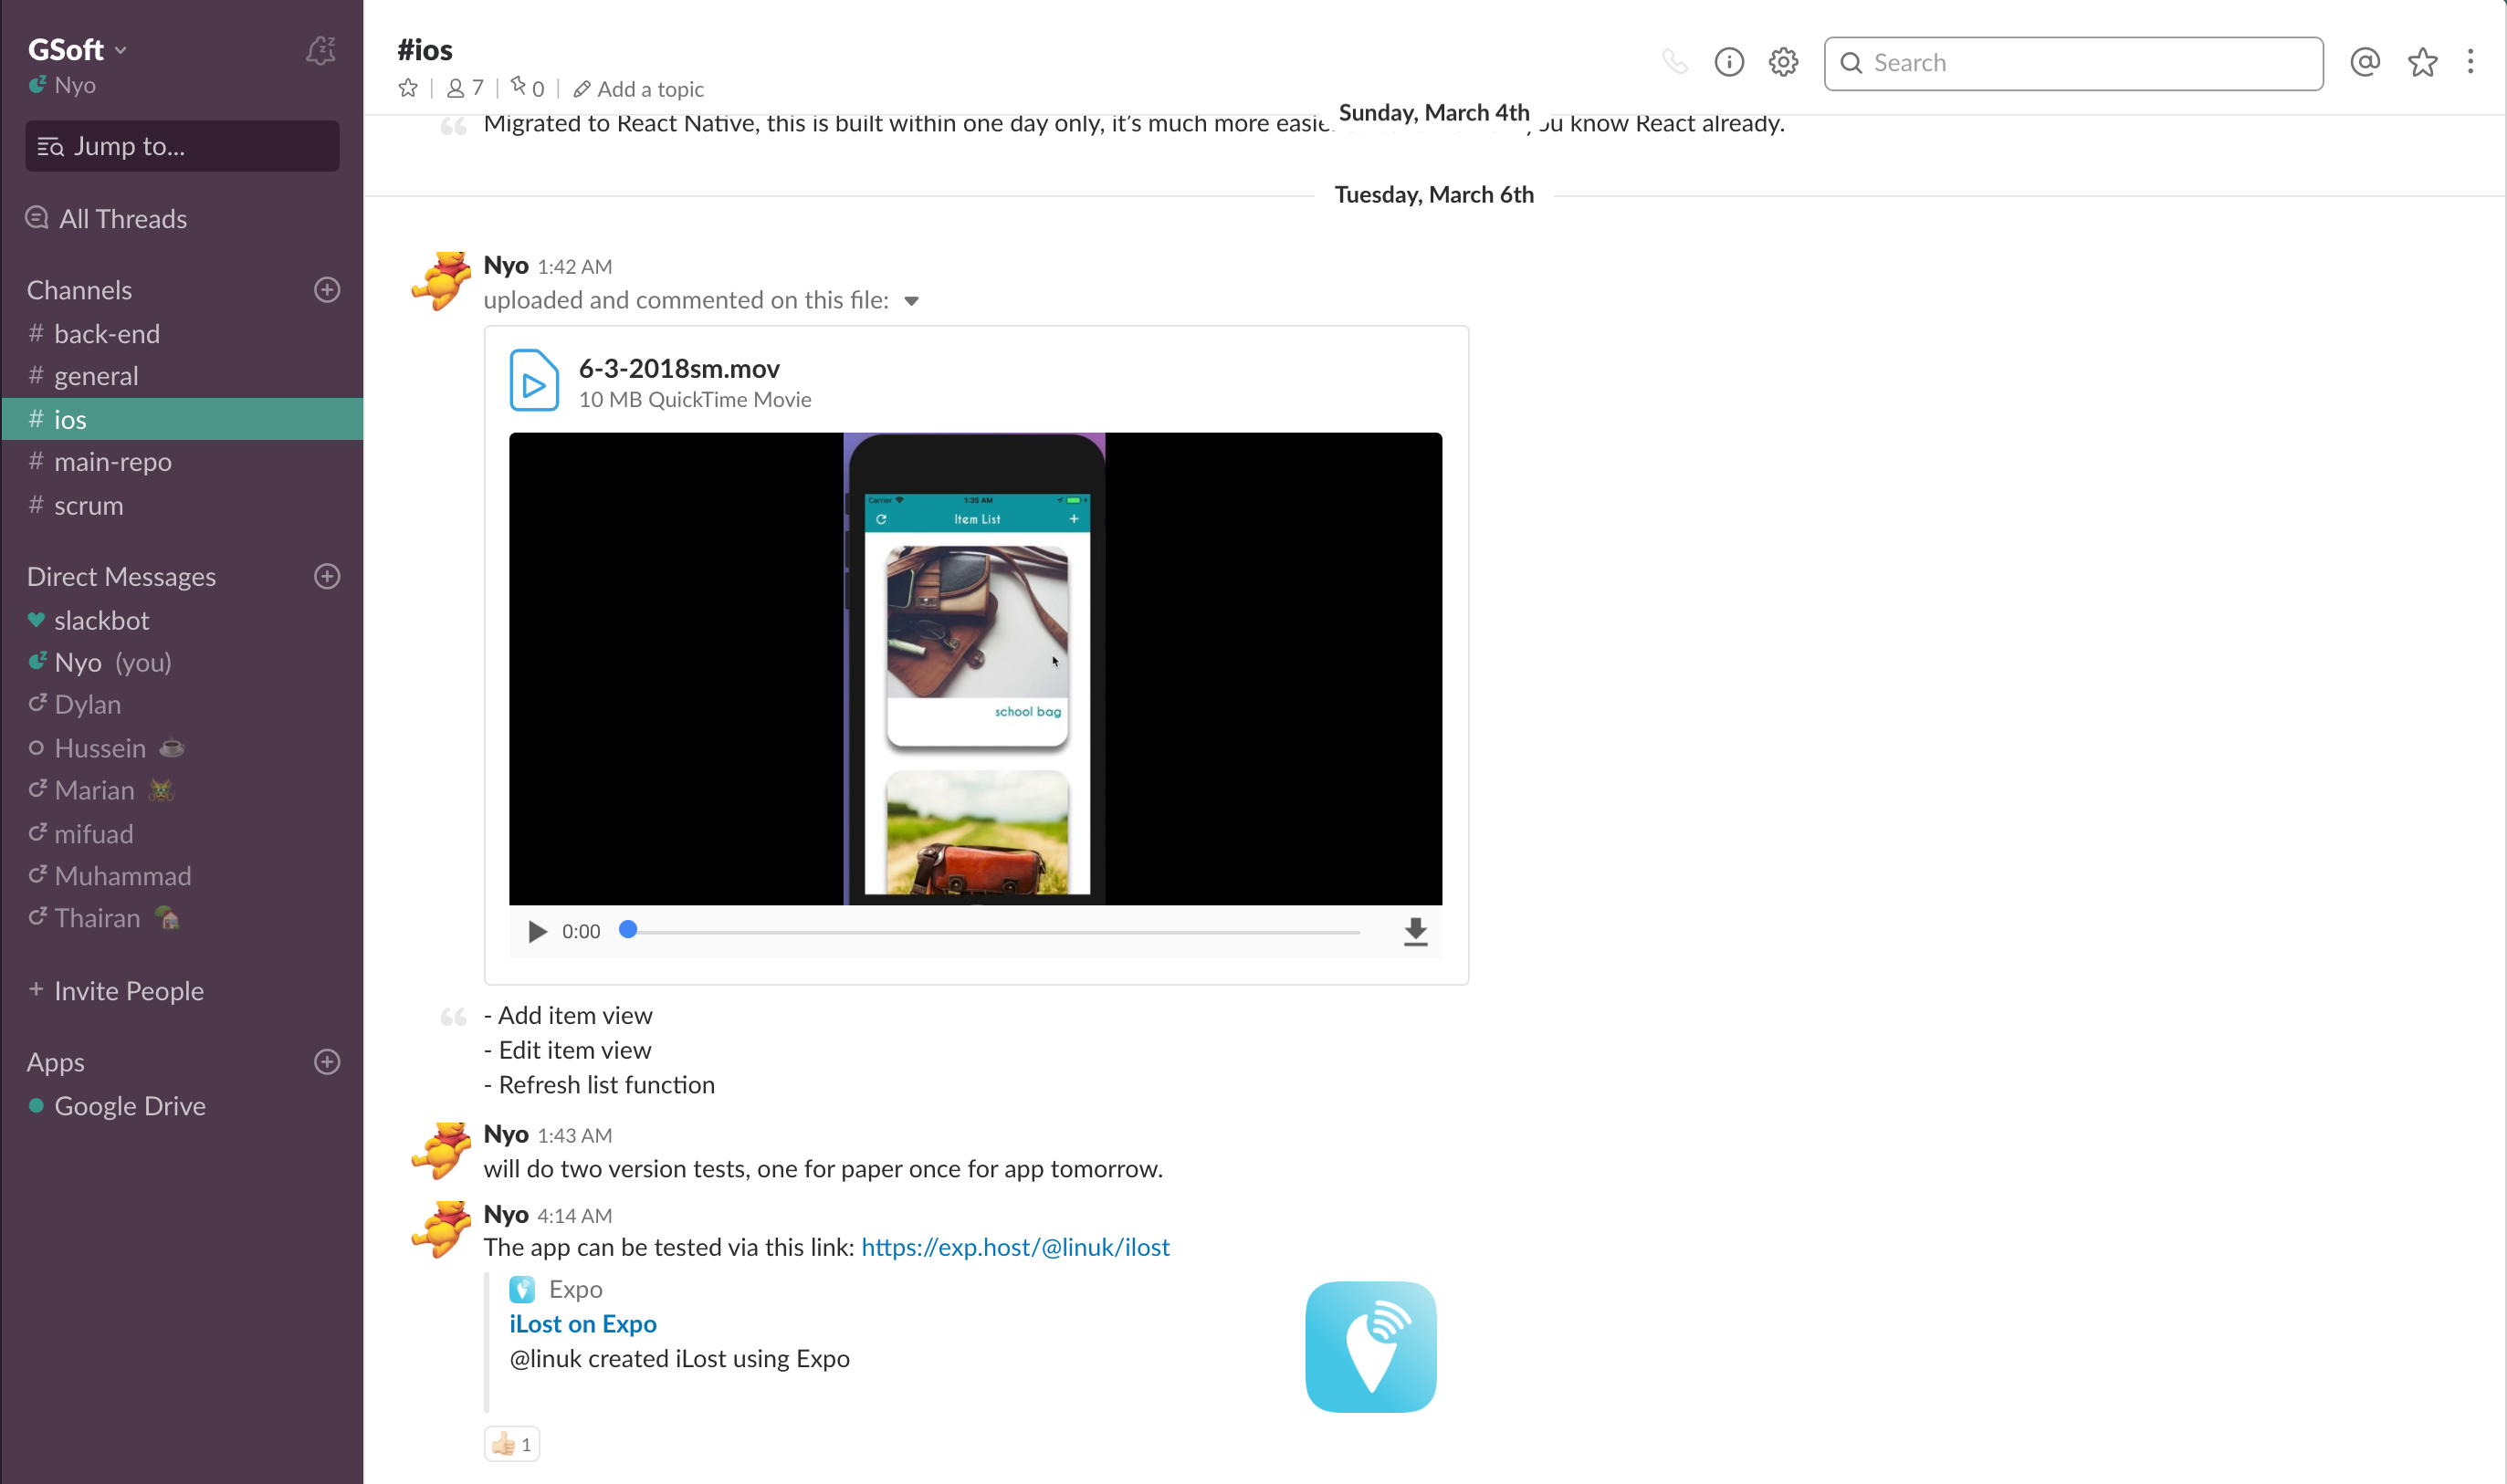
\includegraphics[width=1\textwidth]{../assets/development-records-slack-ios-channel.png}
          \caption{Slack iOS Channel}
          \label{fig:Slack iOS Channel}
        \end{figure}

      \subsection{Agile Development} 
        
        Our team tried out two agile development methodology, {\bf Scrum} and {\bf Kanban}. Overall, Scrum was not was not really fit our case and Kanban worked fine.

        \subsubsection{Scrum Development}
        Since we could not actually devote all of our time to develop the application, so it would not be reasonable to do the daily scrum and have a meeting day-to-day for all of us. So in the beginning, we tried to set up a routine to simulate the daily scrum with Slack:

        We defined 3 days as one sprint and whenever a sprint was finished, the team needed to answer three questions in the Scrum channel on Slack:
        
        \begin{itemize}
          \item What did I complete last time that contributed to the team meeting our sprint goal?
          \item What do I plan to complete this time to contribute to the team meeting our sprint goal?
          \item Do I see any impediment that could prevent me or the team from meeting our sprint goal?
        \end{itemize}    

        This was another way to keep everyone updated, but unfortunately, not every team could follow the sprint process and make any progress every three days. Sometimes a team might work for this sprint then stopped for two sprints since other modules might have a deadline or coursework. Hence, this scrum process was not actually conducted properly and stopped after few weeks after started. The records show in figure \ref{fig:Slack Scrum Channel}. 

        \begin{figure}[H]
          \centering
          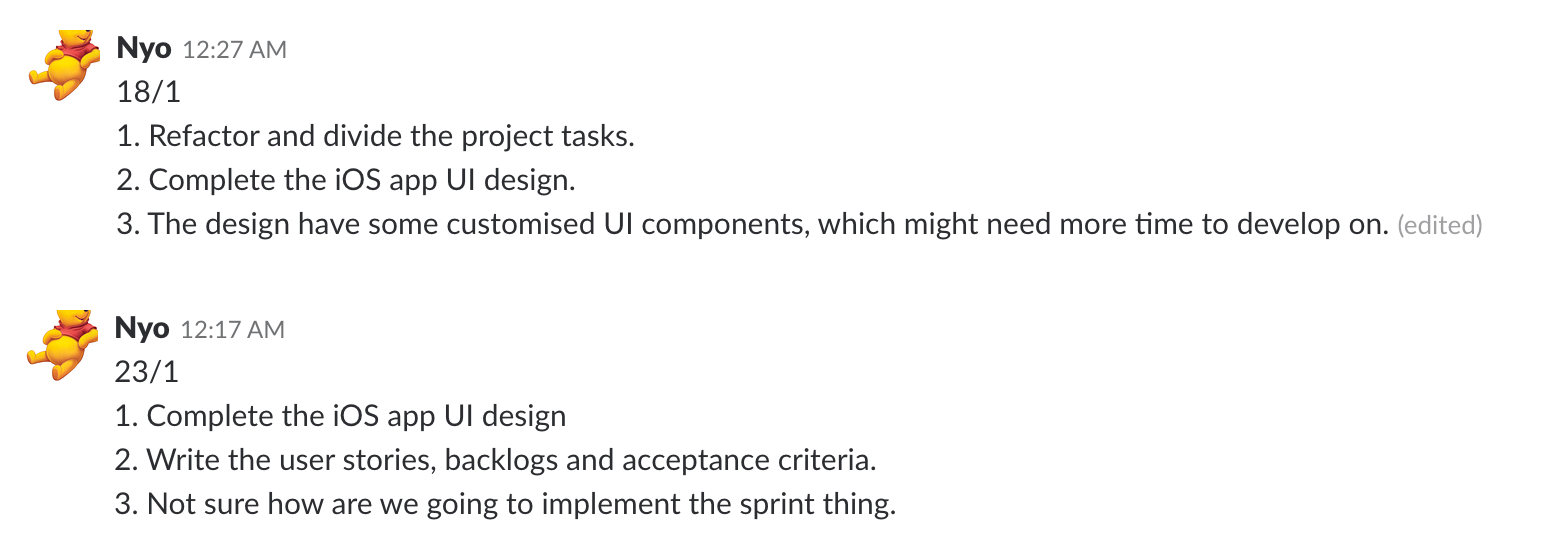
\includegraphics[width=1\textwidth]{../assets/development-records-slack-scrum-channel.png}
          \caption{Slack Scrum Channel}
          \label{fig:Slack Scrum Channel}
        \end{figure}
        
        At the middle of the development stage, our supervisor suggested us to meet 2 hours a day and 2 to 4 days a week, work and team and engage the team building, since the progress tracking form showed that the working hours were really unbalanced and some people apparently did not put enough effort into the project. 
        
        We made a daily sprint schedule, shows in figure \ref{fig:Daily Sprint}, and followed the time to do work together. Everyone should follow the schedule and spend at least two days a week to work together as a team. It went well and most of us were able to follow the schedule. We worked in RHB306a, 35 Cafe or the whitehead building lab. But since the strike started, the daily sprint stopped again because not all of us were coming to the campus due to the long distance between home and the university. 

        \begin{figure}[H]
          \centering
          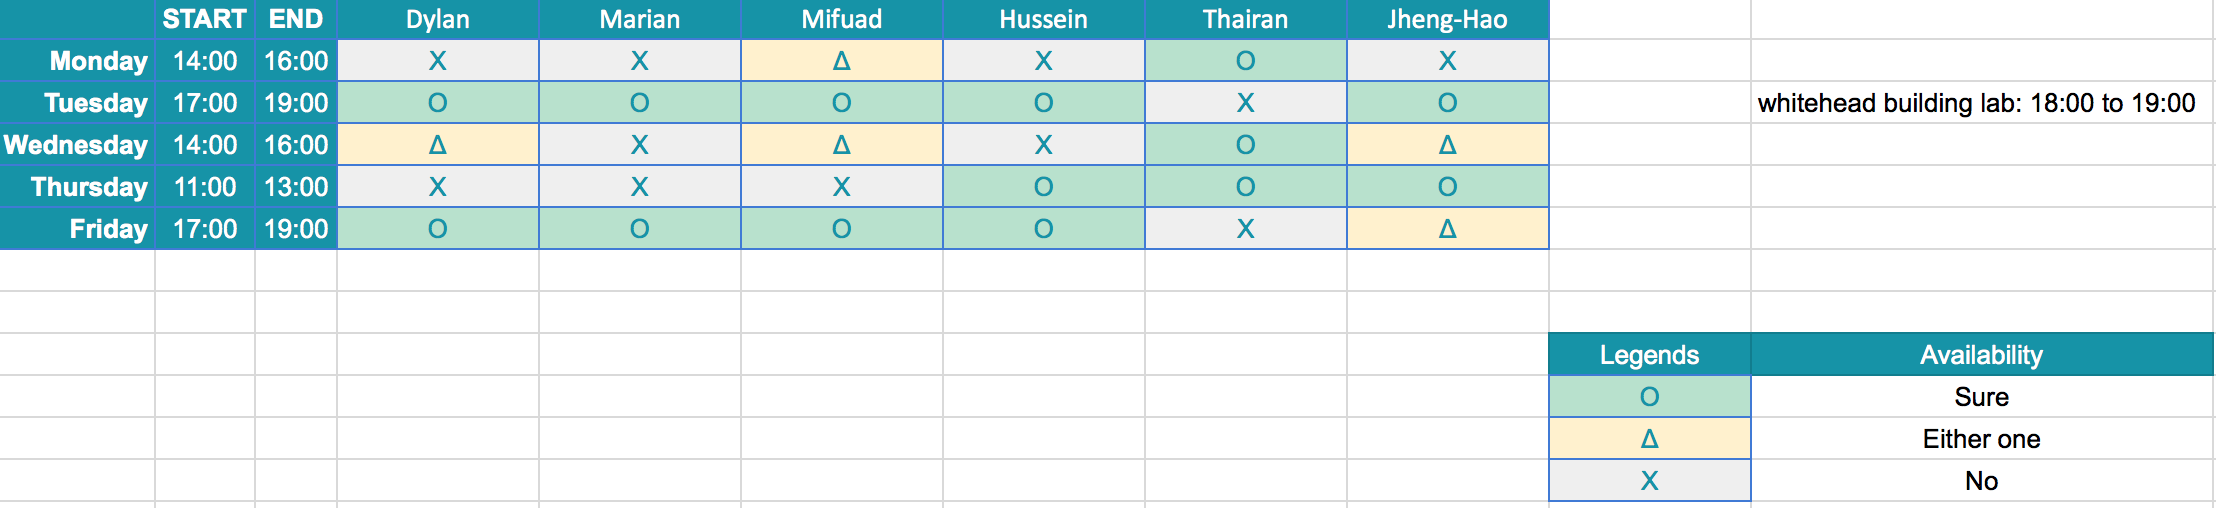
\includegraphics[width=1\textwidth]{../assets/development-records-daily-sprint.png}
          \caption{Daily Sprint}
          \label{fig:Daily Sprint}
        \end{figure}

        \subsubsection{Kanban}
          Apart from the Scrum, Kanban was also implemented with the backlogs in our development to demonstrate the development progress. We tried to keep our project management tool simple and easy to approach, so we not only used Github for version control but also for the project feature, which we used it as the Kanban. The iOS  development kanban was shown in \ref{fig:iOS Development Kanban}.

          \begin{figure}[H]
            \centering
            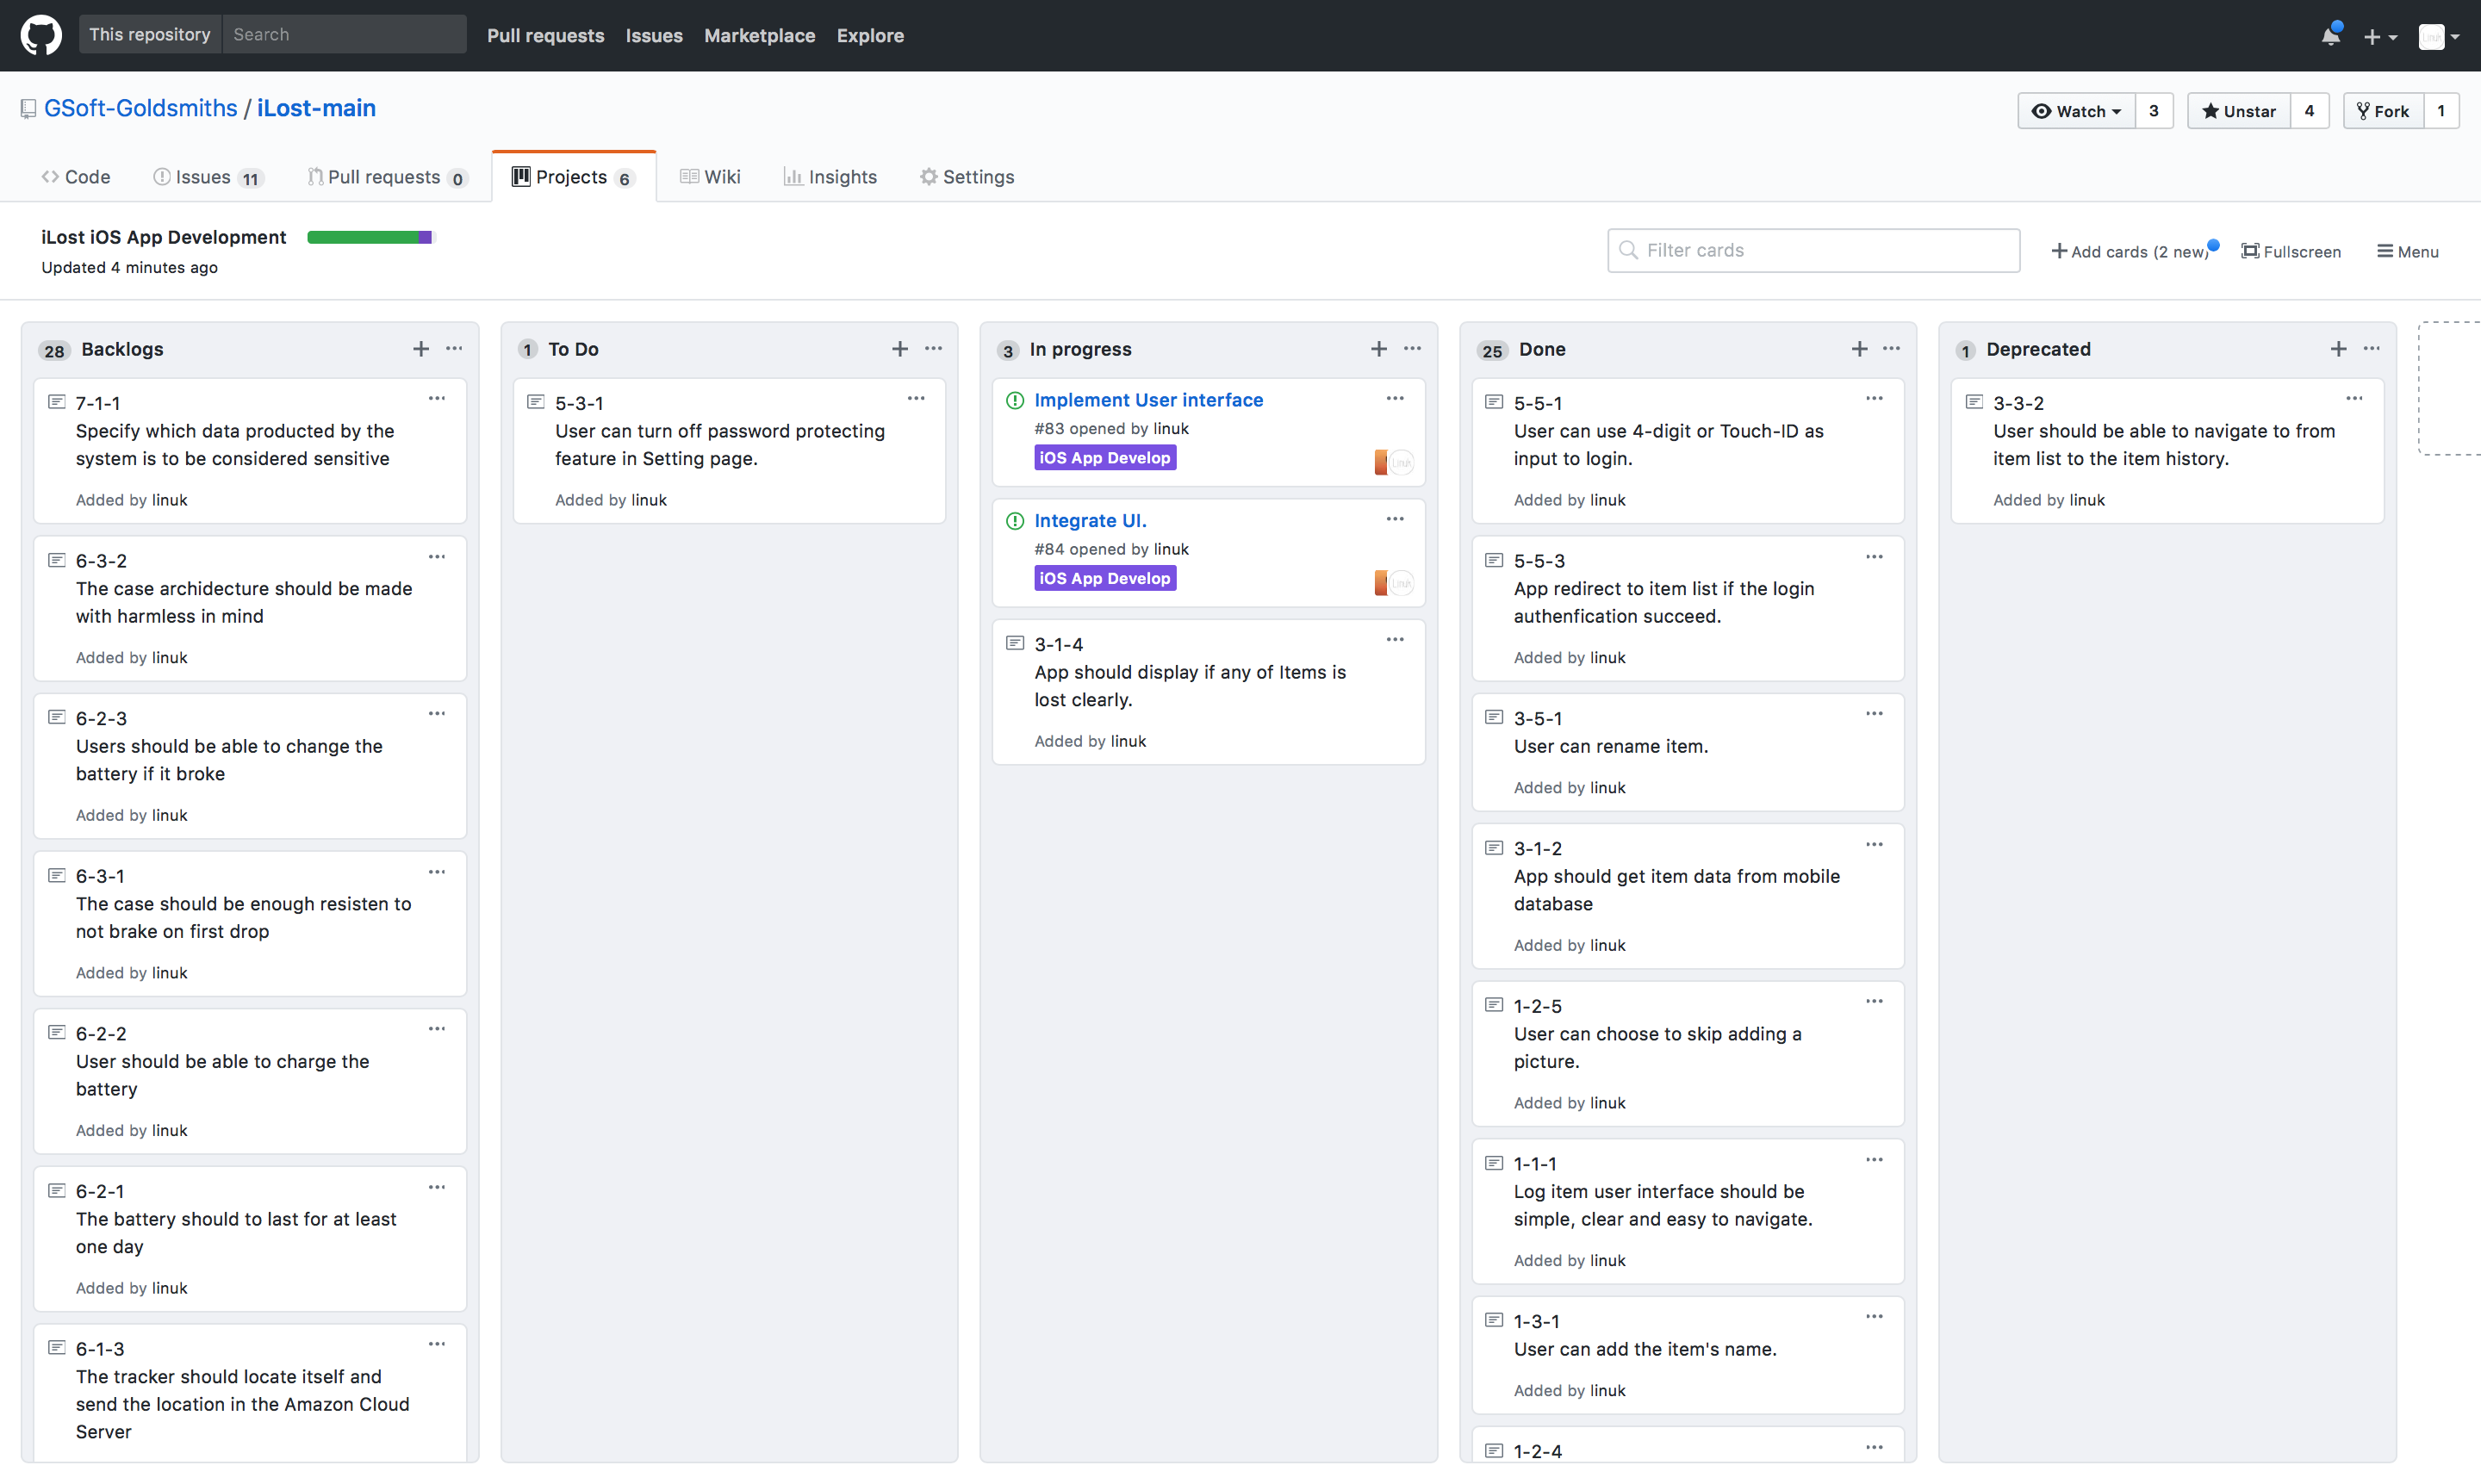
\includegraphics[width=1\textwidth]{../assets/development-records-ios-kanban.png}
            \caption{iOS app Kanban}
            \label{fig:iOS Development Kanban}
          \end{figure}
         
          Our kanban contained five columns which shows in Table \ref{table:Kanban Columns}:
          
          \begin{table}[H]
            \centering
              \begin{tabularx}{\textwidth}{l X}
                \hline
                Column & Description  \\ \hline
                Backlogs & The task is scheduled to be develop, but it is possible to be assigned deprecated if it is no longer needed. \\ 
                To Do & The task is going to be develop.  \\ 
                In Progress & The task is currently developing  \\ 
                Done & The task has been completed.   \\ 
                Deprecated & The task no longer need to be developed.\\                  
                \hline
              \end{tabularx}
              \caption[Table caption text]{Kanban Columns}
              \label{table:Kanban Columns}
          \end{table}
          
          Apart from the normal columns: To Do, In Progress and Done, we also added {\bf Deprecated} to store the features or tasks did not fit the needs anymore. Kanban gave a nice and clean overview of the current developing process, especially for people from other teams.
        
      \subsection{Development Process}
        % 400 - 500 words
        \subsubsection{User Stories and Backlogs}
          Based on the user stories, we setup several backlogs for each user story.
        \subsubsection{Progress Tracking Form}
      \subsection{Evaluation}
        \paragraph{Technology Selection}
        \paragraph{Agile Development}
        \paragraph{Development Progress}
        % 400 - 500 words
    \newpage
    \section{Formative Evaluation}
      % total 1650 words
      \subsection{iOS App Evaluation} 
          % total 1000 words
        \subsubsection{Objectives and Questions}
          % 100 words
          \paragraph{}
            We wrote quantitative tasks to test the usability of our mobile application\cite{WritingTasks}. The purpose of the tests was to test if the participants can actually finish the task with the application, and we could learn from the process to observe how users used our application and improve it if any issue or confusion was raised. 

            \begin{figure}[H]
              \centering
              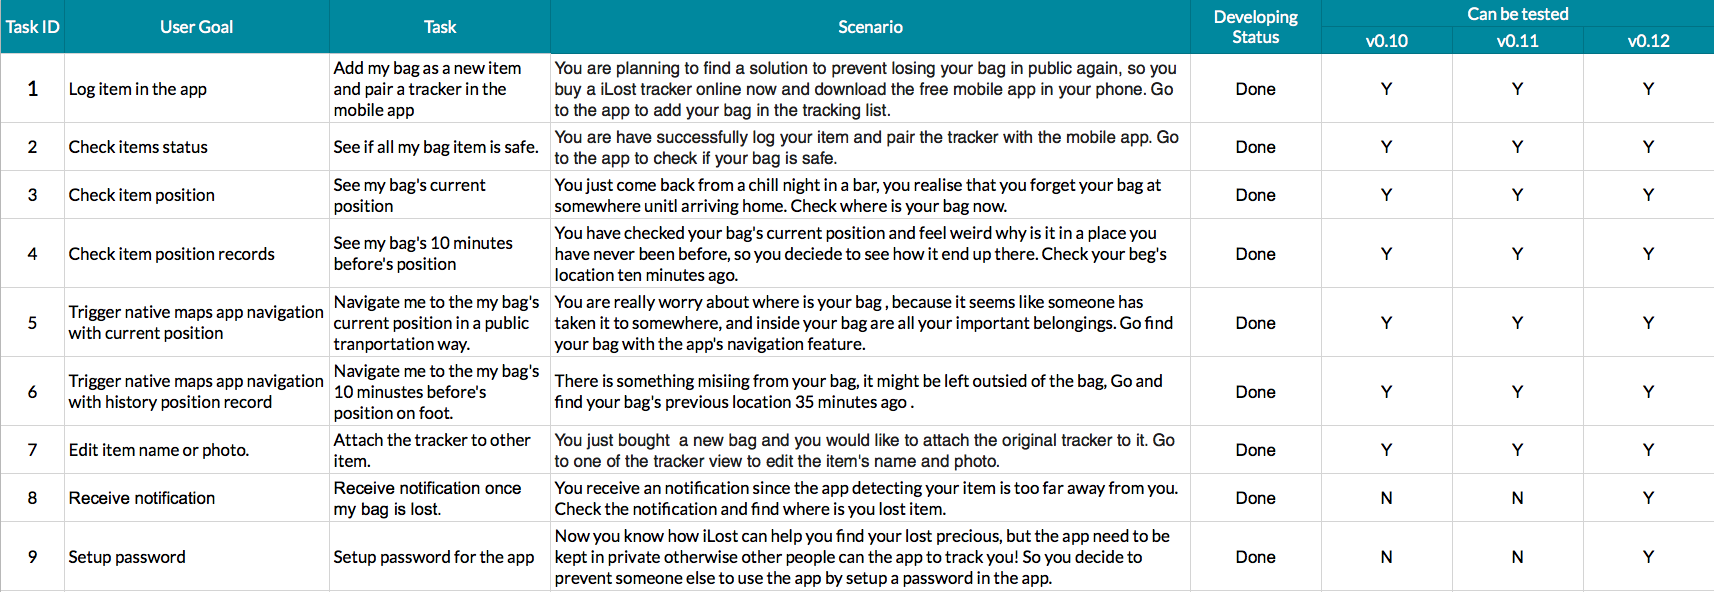
\includegraphics[width=1\textwidth]{../assets/usability-test-task-list.png}
              \caption{Usability test task list}
              \label{fig:Usability test task list}
            \end{figure}

            \begin{table}[H]
              \centering
                \begin{tabularx}{\textwidth}{l X}
                  \hline
                  Column & Description  \\ \hline
                  Task ID & Identify number of the task  \\ 
                  User Goal & What is the objective we need users to perform.  \\ 
                  Task & The process in terms of completing the goal  \\ 
                  Scenario & A setup scenario for engaging testers to use the application in a real-life case.   \\ 
                  Developing Status & Current latest developing status of the functionality of this task, it should be {\bf To do}, {\bf In Progress} and {\bf Done}.\\ 
                  Can be tested &  Whether the functionality of the application is ready to be tested in each version.\\ 
                  \hline
                \end{tabularx}
                \caption[Table caption text]{Usability test task list columns}
                \label{table:Usability test task list columns}
            \end{table}

            Figure \ref{fig:Usability test task list} demonstrates our tasks and goals. The table \ref{table:Usability test task list columns} shows what the columns stand for.

        \subsubsection{Participants, Location and Setup}
          % 100 words
          \paragraph{} According to Jakob Nielsen, testing 5 users in a usability study could find almost as many usability problems as testing more participants\cite{HowManyTestUsers}. So application was tested with 5 participants for each version. The study was taken place in the library of the Goldsmiths, University of London, and the participants were the students who used to bring a bag to the campus daily. Totally we have conducted three versions of the application.
          
        \subsubsection{Methodology and Measures}
          % 100 words
          \paragraph{} Firstly, we explained what was our project about and asked participants to sign up the consent form which can be found in appendices \ref{appendix:consent-form}. During the test, the participants were provided an iPhone with the application built-in to test. An observer would guide them through the tasks and the scenarios, then took notes of how the participants reacted to the application. For each task, the observer would record it was successfully completed or failed. The records would help us to build the success rates diagram which helped us to understand which usability needed to be improved\cite{SuccessRates}. 

        
        \subsubsection{Evaluation}
          
          \begin{figure}[H]
            \centering
            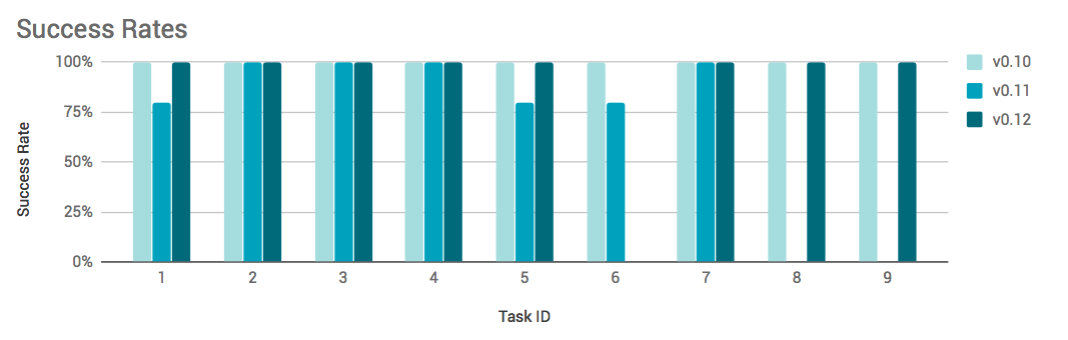
\includegraphics[width=1\textwidth]{../assets/usability-test-success-rates.png}
            \caption{iOS App Success Rates Diagram}
            \label{fig:iOS App Success Rates Diagram}
          \end{figure}

          \paragraph{v0.10} The tested subject was the application prototype built in {\bf Adobe XD}, which was one of the best design tools to test the prototype. Thanks to the well-designed user interfaces, the goals were easy to achieved and all the tasks were all succeeded. The result could only prove that the user interfaces guided the users to the right view, but it could not actually reflect on the usability of the real application. After all, Adobe XD could only let users walk through each view by clicking, while an actual iOS application should support swipe or other gestures. It was more like a paper prototype usability test.
          
          \paragraph{v0.11} We benefited most from this test since this test was the native mobile application we where the participants can actually use it like other application. This version was built in React Native and tested in Expo which a tool and service which we used to build the mobile native application with React Native. During this test, we received several comments towards the {\bf add item view}. For example, the camera icon in that view was originally used as a button. But some of the users could not really regard it as a button but a decoration since it was colourful. Also, the placeholder of the item name field was {\bf Item Name} instead of a prompt message which confused some of the participants as well. So after this test, we resolved the issues and the difference shows in figure \ref{fig:usability-test-ios-v010-improvements}. The task 8 and 9 were not developed completely at the moment so there was not any record.

          \begin{figure}[H]
            \centering
            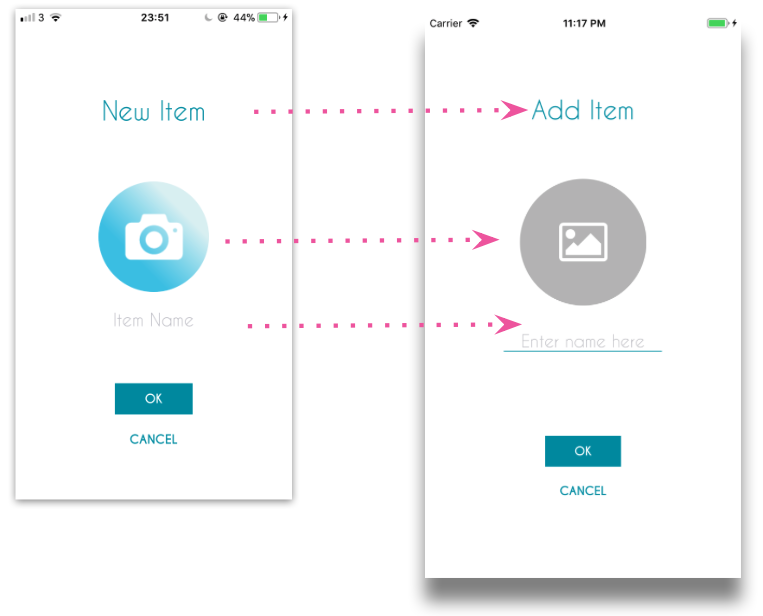
\includegraphics[width=0.7\textwidth]{../assets/usability-test-ios-v010-improvements.png}
            \caption{Improvement of the add item view}
            \label{fig:usability-test-ios-v010-improvements}
          \end{figure}

          \paragraph{v0.12} After the previous test, we not only improved some of the user interfaces but also removed some of the features. It is worth notice that there is no record of task 6, which is {\bf navigating to previous locations of the item's location history}. The reason we removed this task was that this goal was not really helpful. The participants commented that it was not beneficial to navigate to the previous locations, they cared about the current location of the item more. So thanks to the feedback, we removed the task 6 and eliminated the functionality of navigating through history locations which made the application more simple. 
        
        \subsection{Tracker Evaluation}
            total 700 words
          \subsubsection{Objectives and Questions}
            100 words
          \subsubsection{Location, Setup and Participants}
            100 words
          \subsubsection{Methodology and Measures}
            100 words
          \subsubsection{Tracker v0.10 Evaluation}
            150 max words
          \subsubsection{Tracker v0.11 Evaluation}
            150 max words
        \subsection{Conclusion}
          % 200 max words
          Even though the tasks could be completed, but in terms of the user experience, we still had space to improved. 
      \newpage
    \section{Design and Implementation}
    \section{Quality Assurance}
    \section{Summative Evaluation}
    
    \begin{thebibliography}{20}
      % \addcontentsline{toc}{chapter}{Bibliography}
      \bibitem{HowManyTestUsers} "How Many Test Users in a Usability Study?", Nielsen Norman Group, 2012. [Online]. Available: https://www.nngroup.com/articles/how-many-test-users/. [Accessed: 01- Mar- 2018].
      \bibitem{WritingTasks} "Writing Tasks for Quantitative and Qualitative Usability Studies", Nielsen Norman Group, 2018. [Online]. Available: https://www.nngroup.com/articles/test-tasks-quant-qualitative/. [Accessed: 14- Mar- 2018].
      \bibitem{SuccessRates} "Success Rate: The Simplest Usability Metric", Nielsen Norman Group, 2001. [Online]. Available: https://www.nngroup.com/articles/success-rate-the-simplest-usability-metric/. [Accessed: 14- Mar- 2018].
    \end{thebibliography}
    
    \begin{appendices}            
      \section{Development Records}
        \subsection{Tasks Divided}
        \subsection{Progress Tracking Form}
      \section{Formative Evaluation}
        \subsection{consent Form}
          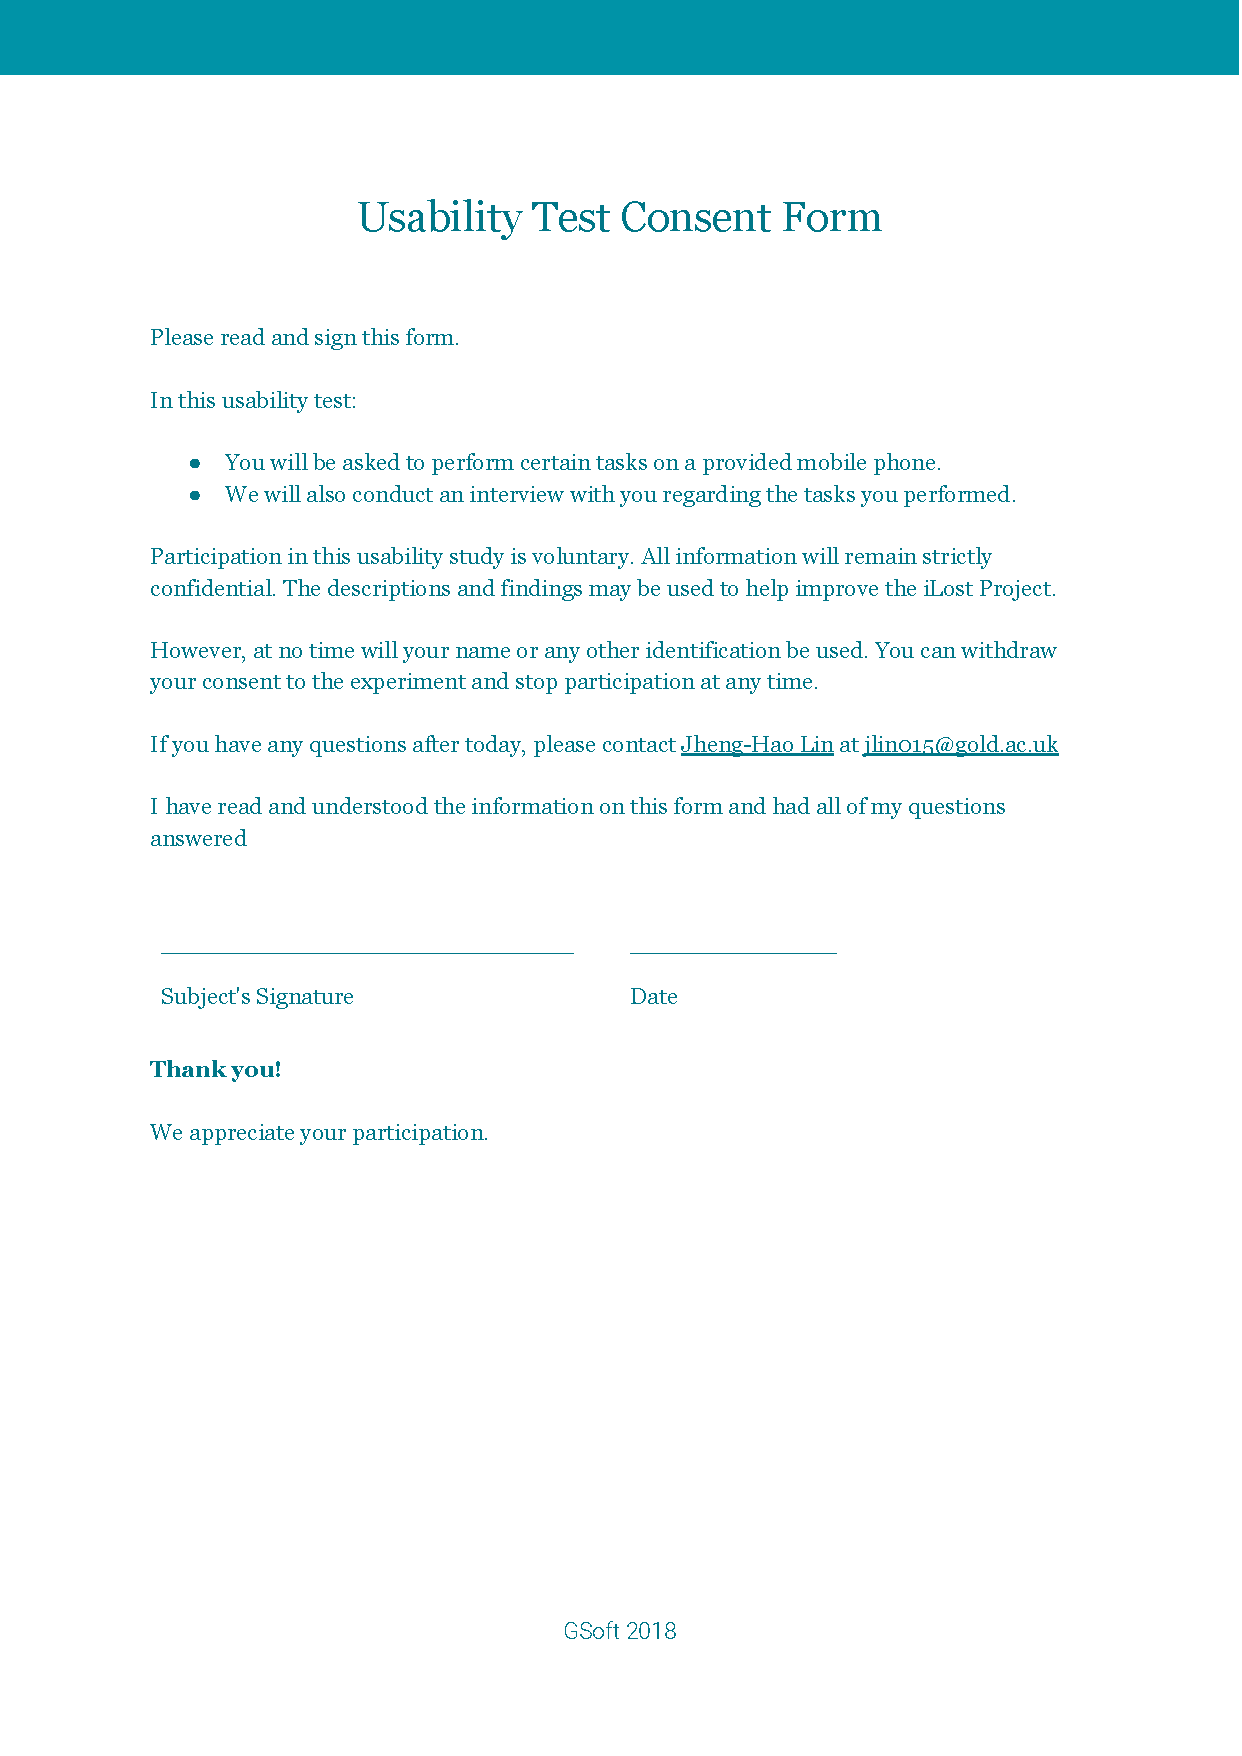
\includepdf[pages={1}]{../assets/usability-test-consent-form-example.pdf}
          \label{appendix:consent-form}
      \section{Design and Implementation}
        
      \section{Quality Assurance}

    \end{appendices}

  \end{document}


